\documentclass[11pt]{article}
\usepackage[margin=1in]{geometry}
\usepackage{amsmath,amssymb}
\usepackage{siunitx}
\usepackage{physics}
\usepackage{tikz}
\usetikzlibrary{arrows.meta,angles,quotes,calc,decorations.pathmorphing,decorations.markings}
\usepackage{enumitem}
\sisetup{per-mode=symbol}

\newcommand{\ans}[1]{\boxed{\displaystyle #1}}

\title{PHYS 121 --- HW5 Solutions}
\author{Juntang Wang}

\begin{document}
\maketitle
\setlist[itemize]{noitemsep,topsep=2pt}

% Helper constants
\def\g{\,\mathrm{g}}

\section*{Q1. Spider silk realism + Spiderman (16 pts)}
Given: Elastic modulus $Y = \SI{25}{GPa} = \SI{2.5e10}{N/m^2}$, spider mass $m = \SI{50}{mg} = \SI{5e-5}{kg}$, line diameter $d = \SI{0.14}{mm} = \SI{1.4e-4}{m}$, length $L = \SI{50}{cm} = \SI{0.50}{m}$.

\textbf{(a) Stretch:} Cross-sectional area: $A = \pi(d/2)^2 = \pi \times (7 \times 10^{-5})^2 = \pi \times 4.9 \times 10^{-9} = \SI{1.54e-8}{m^2}$.

Tension equals weight: $F = mg = 5 \times 10^{-5} \times 9.8 = \SI{4.9e-4}{N}$.

From $F = YA x/L$:
\[ x = \frac{FL}{YA} = \frac{4.9 \times 10^{-4} \times 0.50}{2.5 \times 10^{10} \times 1.54 \times 10^{-8}} = \frac{2.45 \times 10^{-4}}{3.85 \times 10^{2}} = \ans{\SI{6.36e-7}{m} = \SI{0.636}{\micro\meter}}. \]

\textbf{(b) Potential energy:} $U = \frac{1}{2}kx^2$, where effective spring constant $k = YA/L$.

\[ k = \frac{2.5 \times 10^{10} \times 1.54 \times 10^{-8}}{0.50} = \SI{7.7e2}{N/m}. \]

\[ U = \frac{1}{2} \times 770 \times (6.36 \times 10^{-7})^2 = \frac{1}{2} \times 770 \times 4.04 \times 10^{-13} = \ans{\SI{1.56e-10}{J}}. \]

\textbf{(c) Speed:} If all energy converts to kinetic: $\frac{1}{2}mv^2 = U$.

\[ v = \sqrt{\frac{2U}{m}} = \sqrt{\frac{2 \times 1.56 \times 10^{-10}}{5 \times 10^{-5}}} = \sqrt{6.24 \times 10^{-6}} = \ans{\SI{2.50e-3}{m/s} = \SI{2.50}{mm/s}}. \]

\textbf{(d) Drawing:}
\begin{center}
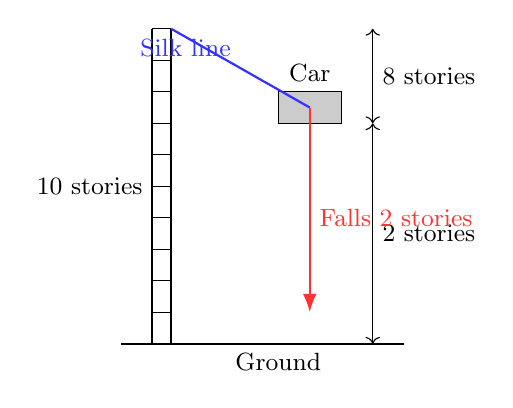
\begin{tikzpicture}[scale=0.8]
  % Parking garage (10 stories)
  \draw[thick] (0,0) -- (0,5);
  \draw[thick] (0.3,0) -- (0.3,5);
  \foreach \y in {0.5,1,1.5,2,2.5,3,3.5,4,4.5,5} {
    \draw (0,\y) -- (0.3,\y);
  }
  \node[left] at (0,2.5) {\small 10 stories};
  % Car falling
  \draw[fill=gray!40] (2,3.5) rectangle (3,4);
  \node[above] at (2.5,4) {\small Car};
  % Silk line
  \draw[thick,blue!80] (0.3,5) -- (2.5,3.75);
  \node[above left,blue!80] at (1.4,4.4) {\small Silk line};
  % Ground
  \draw[thick] (-0.5,0) -- (4,0);
  \node[below] at (2,0) {\small Ground};
  % Height markers
  \draw[<->] (3.5,0) -- (3.5,3.5) node[midway,right] {\small 2 stories};
  \draw[<->] (3.5,3.5) -- (3.5,5) node[midway,right] {\small 8 stories};
  % Arrow showing fall
  \draw[-{Latex},thick,red!80] (2.5,3.75) -- (2.5,0.5);
  \node[right,red!80] at (2.5,2) {\small Falls 2 stories};
\end{tikzpicture}
\end{center}

\textbf{(e) Minimum diameter (infinitely elastic):} Assume story height $\approx \SI{3}{m}$. Car mass $m_{\text{car}} \approx \SI{1500}{kg}$.

Car falls from top (10 stories) and line connects at 2 stories above ground. Distance fallen: $h_{\text{fall}} = 8 \times \SI{3}{m} = \SI{24}{m}$. Speed at connection: $v = \sqrt{2gh_{\text{fall}}} = \sqrt{2 \times 9.8 \times 24} = \SI{21.7}{m/s}$.

Car must stop at ground (additional 2 stories = $\SI{6}{m}$ below connection point). The energy that must be absorbed by the line includes both the kinetic energy at connection and the gravitational potential energy lost as the car falls the additional 6 m:
\[ E_{\text{total}} = \frac{1}{2}mv^2 + mgh_{\text{stop}} = \frac{1}{2} \times 1500 \times (21.7)^2 + 1500 \times 9.8 \times 6 = 353000 + 88200 = \SI{4.41e5}{J}. \]

If the line is infinitely elastic and stretches by $x = \SI{6}{m}$ (the distance car falls after connection), the energy stored is $U = \frac{1}{2}kx^2$, where $k = YA/L_0$.

Assuming the line's unstretched length is approximately the connection height ($L_0 \approx \SI{6}{m}$), then:
\[ U = \frac{1}{2} \cdot \frac{YA}{L_0} \cdot x^2 = \frac{1}{2} \cdot \frac{YA}{6} \cdot 36 = 3YA. \]

Setting $U = E_{\text{total}} = \SI{4.41e5}{J}$:
\[ 3 \times 2.5 \times 10^{10} \times A = 4.41 \times 10^5 \quad\Rightarrow\quad A = \frac{4.41 \times 10^5}{7.5 \times 10^{10}} = \SI{5.88e-6}{m^2}. \]

\[ d = 2\sqrt{\frac{A}{\pi}} = 2\sqrt{\frac{5.88 \times 10^{-6}}{\pi}} = 2\sqrt{1.87 \times 10^{-6}} = 2 \times 1.368 \times 10^{-3} = \ans{\SI{2.74e-3}{m} = \SI{2.74}{mm}}. \]

\textbf{(f) Would the line break?} Real silk has a breaking stress. Typical spider silk breaking stress $\sigma_{\text{max}} \approx \SI{1}{GPa} = \SI{1e9}{Pa}$ (dragline silk can be higher, up to $\sim\SI{1.3}{GPa}$, but we'll use $\SI{1}{GPa}$).

Using the area from part (e): $A = \SI{5.88e-6}{m^2}$.

Maximum tension: $F_{\text{max}} = \sigma_{\text{max}} A = 1 \times 10^9 \times 5.88 \times 10^{-6} = \SI{5.88e3}{N} = \SI{5880}{N}$.

The tension in the line when stretched by $x$ is $F = kx = \frac{YA}{L_0}x$. For $x = \SI{6}{m}$ and $L_0 = \SI{6}{m}$:
\[ F = \frac{2.5 \times 10^{10} \times 5.88 \times 10^{-6}}{6} \times 6 = 2.5 \times 10^{10} \times 5.88 \times 10^{-6} = \SI{1.47e5}{N}. \]

This far exceeds $F_{\text{max}} = \SI{5.88e3}{N}$, so \ans{the line would break}. 

Even if we assume the line can stretch more (making $k$ smaller), the tension required to stop the car would still be very large. For a constant deceleration, if the car stops over distance $x = \SI{6}{m}$ with initial speed $v = \SI{21.7}{m/s}$:
\[ v^2 = 2ax \quad\Rightarrow\quad a = \frac{v^2}{2x} = \frac{(21.7)^2}{12} = \SI{39.2}{m/s^2} = 4g. \]

Force needed: $F = ma = 1500 \times 39.2 = \SI{5.88e4}{N}$, which is much larger than $F_{\text{max}}$. The silk cannot provide enough force to stop the car safely without exceeding its breaking stress.

\section*{Q2. Floating ball oscillation (10 pts)}
Given: Solid sphere (radius $r$) floats with half its volume submerged.

\textbf{(a) Mass density:} For floating, buoyant force equals weight. If half volume is submerged:
\[ \rho_{\text{water}} g \cdot \frac{V}{2} = \rho_{\text{ball}} g V \quad\Rightarrow\quad \rho_{\text{ball}} = \frac{\rho_{\text{water}}}{2} = \ans{\SI{500}{kg/m^3}}. \]

\textbf{Required drawing:}
\begin{center}
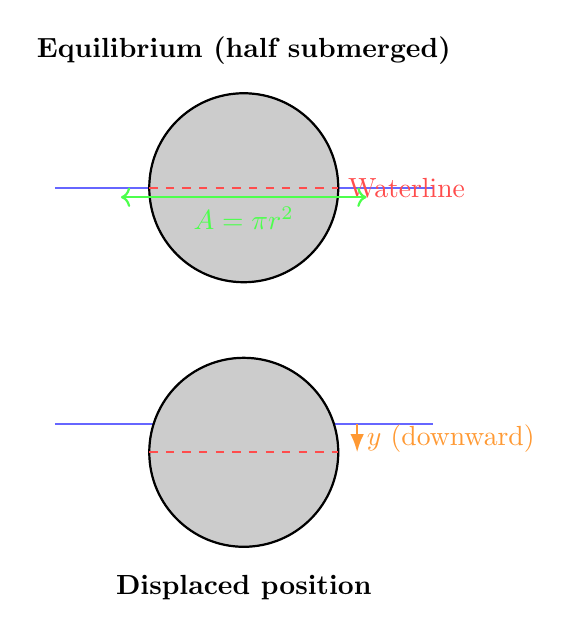
\begin{tikzpicture}[scale=1.2]
  % Water surface
  \draw[thick,blue!60] (-2,0) -- (2,0);
  \node[above,blue!60] at (0,0.1) {Water surface};
  % Sphere at equilibrium (half submerged)
  \draw[fill=gray!40] (0,0) circle (1);
  \draw[thick] (0,0) circle (1);
  % Waterline cross-section
  \draw[dashed,thick,red!70] (-1,0) -- (1,0);
  \node[right,red!70] at (1,0) {Waterline};
  % Cross-sectional area at waterline
  \draw[<->,green!70,thick] (-1.3,-0.1) -- (1.3,-0.1);
  \node[below,green!70] at (0,-0.1) {$A = \pi r^2$};
  % Displacement y downward
  \begin{scope}[yshift=-2.5cm]
    \draw[thick,blue!60] (-2,0) -- (2,0);
    \draw[fill=gray!40] (0,-0.3) circle (1);
    \draw[thick] (0,-0.3) circle (1);
    \draw[dashed,thick,red!70] (-1,-0.3) -- (1,-0.3);
    % Displacement arrow
    \draw[-{Latex},thick,orange!80] (1.2,0) -- (1.2,-0.3);
    \node[right,orange!80] at (1.2,-0.15) {$y$ (downward)};
    \node[below] at (0,-1.5) {\textbf{Displaced position}};
  \end{scope}
  \node[above] at (0,1.2) {\textbf{Equilibrium (half submerged)}};
\end{tikzpicture}
\end{center}

\textbf{(b) SHM and frequency:} When displaced downward by $y$ (small), the additional submerged volume is approximately $\Delta V = \pi r^2 y$ (for small $y$, the cross-section at waterline is $\pi r^2$).

Additional buoyant force: $\Delta F_b = \rho_{\text{water}} g \pi r^2 y$.

Net restoring force: $F = -\rho_{\text{water}} g \pi r^2 y = -ky$, where $k = \rho_{\text{water}} g \pi r^2$.

Newton's second law: $m \frac{d^2y}{dt^2} = -ky$.

This is SHM with angular frequency: $\omega = \sqrt{\frac{k}{m}} = \sqrt{\frac{\rho_{\text{water}} g \pi r^2}{m}}$.

Mass of ball: $m = \rho_{\text{ball}} V = \rho_{\text{ball}} \cdot \frac{4}{3}\pi r^3 = \frac{\rho_{\text{water}}}{2} \cdot \frac{4}{3}\pi r^3 = \frac{2}{3}\pi r^3 \rho_{\text{water}}$.

\[ \omega = \sqrt{\frac{\rho_{\text{water}} g \pi r^2}{\frac{2}{3}\pi r^3 \rho_{\text{water}}}} = \sqrt{\frac{3g}{2r}}. \]

Frequency: $f = \frac{\omega}{2\pi} = \ans{\frac{1}{2\pi}\sqrt{\frac{3g}{2r}}}$.

\textbf{(c) Scaling with viscous drag:} If viscous drag matters, the drag force scales as $F_d \propto \eta r v$ (Stokes' law for small Reynolds number), where $\eta$ is viscosity and $v$ is velocity.

The restoring force scales as $F_r \propto r^2 y$ (from $k = \rho g \pi r^2$).

For small $r$, drag becomes more significant relative to restoring force. The effective damping increases, reducing the oscillation frequency. As $r$ decreases, the frequency \ans{decreases} because viscous effects become more dominant relative to the buoyant restoring force.

\section*{Q3. Challenger Deep (13 pts)}
Given: Bathyscaphe Trieste at depth $h = \SI{10900}{m}$, steel sphere outside diameter $D = \SI{2.16}{m}$ (radius $R = \SI{1.08}{m}$), salt water density $\rho_{\text{sw}} = \SI{1030}{kg/m^3}$, atmospheric pressure $P_0 = \SI{101325}{Pa}$.

\textbf{(a) Pressure difference:} Outside pressure: $P_{\text{out}} = P_0 + \rho_{\text{sw}} g h = 101325 + 1030 \times 9.8 \times 10900$.

\[ P_{\text{out}} = 101325 + 1.100 \times 10^8 = \SI{1.101e8}{Pa} = \SI{110.1}{MPa}. \]

Inside pressure: $P_{\text{in}} = P_0 = \SI{101325}{Pa}$ (atmospheric).

Pressure difference: $\Delta P = P_{\text{out}} - P_{\text{in}} = \ans{\SI{1.10e8}{Pa} = \SI{110}{MPa}}$ (to 3 significant figures).

\textbf{(b) Force on hemispheres:} If the sphere is divided into two hemispheres, the force pushing them together is the pressure difference times the cross-sectional area of the cut.

Cross-sectional area: $A = \pi R^2 = \pi \times (1.08)^2 = \SI{3.66}{m^2}$.

Force: $F = \Delta P \times A = 1.100 \times 10^8 \times 3.66 = \ans{\SI{4.03e8}{N}}$.

\textbf{(c) Minimum shell thickness:} Given compressive yield strength $\sigma_y = \SI{520}{MPa} = \SI{5.20e8}{Pa}$.

For a thin-walled sphere under external pressure, the stress is approximately: $\sigma = \frac{\Delta P R}{2t}$, where $t$ is the thickness.

For safety: $\sigma \leq \sigma_y$, so:
\[ \frac{\Delta P R}{2t} \leq \sigma_y \quad\Rightarrow\quad t \geq \frac{\Delta P R}{2\sigma_y}. \]

\[ t \geq \frac{1.100 \times 10^8 \times 1.08}{2 \times 5.20 \times 10^8} = \frac{1.188 \times 10^8}{1.04 \times 10^9} = \ans{\SI{0.114}{m} = \SI{11.4}{cm}}. \]

\textbf{(d) Mass of shell:} Actual thickness $t = \SI{13}{cm} = \SI{0.13}{m}$, steel density $\rho_{\text{steel}} = \SI{7800}{kg/m^3}$.

Volume of shell: $V_{\text{shell}} = \frac{4}{3}\pi[(R+t)^3 - R^3] = \frac{4}{3}\pi[(1.08+0.13)^3 - (1.08)^3]$.

\[ V_{\text{shell}} = \frac{4}{3}\pi[(1.21)^3 - (1.08)^3] = \frac{4}{3}\pi[1.771 - 1.260] = \frac{4}{3}\pi \times 0.511 = \SI{2.14}{m^3}. \]

Mass: $m = \rho_{\text{steel}} V_{\text{shell}} = 7800 \times 2.14 = \ans{\SI{16700}{kg} = \SI{16.7}{tonnes}}$.

\textbf{(e) Gasoline volume for neutral buoyancy:} Gasoline density $\rho_{\text{gas}} = \SI{750}{kg/m^3}$.

For neutral buoyancy, the total weight equals the buoyant force. The bathyscaphe's mass is either gasoline or the metal shell.

Buoyant force: $F_b = \rho_{\text{sw}} g V_{\text{displaced}}$, where $V_{\text{displaced}}$ is the volume of the sphere plus the gasoline float.

If we assume the gasoline is in a separate float tank, and the total displaced volume includes both the sphere and gasoline, then for neutral buoyancy:
\[ m_{\text{total}} g = \rho_{\text{sw}} g V_{\text{total}}. \]

The sphere volume: $V_{\text{sphere}} = \frac{4}{3}\pi R^3 = \frac{4}{3}\pi (1.08)^3 = \SI{5.28}{m^3}$.

If the gasoline volume is $V_{\text{gas}}$, and assuming the gasoline float has negligible volume compared to the gasoline itself, then:
\[ m_{\text{shell}} + \rho_{\text{gas}} V_{\text{gas}} = \rho_{\text{sw}}(V_{\text{sphere}} + V_{\text{gas}}). \]

\[ 16700 + 750 V_{\text{gas}} = 1030(5.28 + V_{\text{gas}}) = 5438 + 1030 V_{\text{gas}}. \]

\[ 16700 - 5438 = 1030 V_{\text{gas}} - 750 V_{\text{gas}} = 280 V_{\text{gas}}. \]

\[ V_{\text{gas}} = \frac{11262}{280} = \ans{\SI{40.2}{m^3}}. \]

\section*{Q4. More on air pressure (15 pts)}
Given: $P_0 = \SI{100}{kPa} = \SI{1e5}{Pa}$ at sea level, $\rho_0 = \SI{1.2}{kg/m^3}$.

\textbf{(a) Constant density model - atmosphere depth:} Using hydrostatic equation: $dP/dz = -\rho g$.

With constant density: $P(z) = P_0 - \rho_0 g z$.

At the top of the atmosphere, $P = 0$, so:
\[ 0 = P_0 - \rho_0 g H \quad\Rightarrow\quad H = \frac{P_0}{\rho_0 g} = \frac{1 \times 10^5}{1.2 \times 9.8} = \ans{\SI{8507}{m} \approx \SI{8.5}{km}}. \]

\textbf{(b) Mountain pressure (constant density):} For mountain height $z = \SI{7700}{m}$:
\[ P = P_0 - \rho_0 g z = 1 \times 10^5 - 1.2 \times 9.8 \times 7700 = 1 \times 10^5 - 90552 = \ans{\SI{9448}{Pa} = \SI{9.45}{kPa}}. \]

\textbf{(c) Variable density model:} If density is proportional to pressure: $\rho = \rho_0 \frac{P}{P_0}$.

From hydrostatic equation: $\frac{dP}{dz} = -\rho g = -\rho_0 \frac{P}{P_0} g$.

Rearranging: $\frac{dP}{P} = -\frac{\rho_0 g}{P_0} dz$.

Integrating: $\ln P = -\frac{\rho_0 g}{P_0} z + C$.

At $z = 0$, $P = P_0$, so $C = \ln P_0$.

\[ \ln\left(\frac{P}{P_0}\right) = -\frac{\rho_0 g}{P_0} z \quad\Rightarrow\quad P = P_0 e^{-z/\alpha}, \]
where $\alpha = \frac{P_0}{\rho_0 g}$.

\textbf{(d) Dimensions of $\alpha$:} $\alpha = \frac{P_0}{\rho_0 g} = \frac{\text{Pa}}{\text{kg/m}^3 \times \text{m/s}^2} = \frac{\text{N/m}^2}{\text{kg/(m}^2 \text{s}^2)} = \text{m}$. So $\alpha$ has dimensions of \ans{length (meters)}.

\textbf{(e) Numerical value of $\alpha$:}
\[ \alpha = \frac{P_0}{\rho_0 g} = \frac{1 \times 10^5}{1.2 \times 9.8} = \ans{\SI{8507}{m} \approx \SI{8.5}{km}}. \]

This is the scale height of the atmosphere.

\textbf{(f) Mountain pressure (variable density):} For $z = \SI{7700}{m}$:
\[ P = P_0 e^{-z/\alpha} = 1 \times 10^5 \times e^{-7700/8507} = 1 \times 10^5 \times e^{-0.905} = 1 \times 10^5 \times 0.4044 = \ans{\SI{40400}{Pa} = \SI{40.4}{kPa}}. \]

\textbf{(g) Mountain name:} The mountain in Sichuan, about 100 km south of Kangding, that is about 7,700 m tall is \ans{Mount Gongga} (also known as Minya Konka), the highest peak in Sichuan Province.

\section*{Q5. Pump out the water (10 pts)}
Given: Water accumulates at depth $h = \SI{3}{m}$ below waterline, pump power $P = \SI{2500}{W}$.

Power required to pump water: $P = \rho g h \times \text{flow rate} = \rho g h Q$.

Flow rate: $Q = \frac{P}{\rho g h} = \frac{2500}{1000 \times 9.8 \times 3} = \frac{2500}{29400} = \SI{0.0850}{m^3/s}$.

However, this is the theoretical maximum. The actual flow rate depends on pipe diameter due to flow resistance.

\textbf{(a) Pipe diameter $d_1 = \SI{2}{cm} = \SI{0.02}{m}$:} The power required to pump water is $P = \rho g h Q$, where $Q$ is the volumetric flow rate.

Solving for flow rate: $Q = \frac{P}{\rho g h} = \frac{2500}{1000 \times 9.8 \times 3} = \frac{2500}{29400} = \ans{\SI{0.0850}{m^3/s} = \SI{85.0}{L/s}}$.

The flow velocity in the pipe: $v_1 = \frac{Q}{A_1} = \frac{Q}{\pi (d_1/2)^2} = \frac{0.0850}{\pi \times 0.01^2} = \SI{270.6}{m/s}$.

This velocity is very high and would result in significant frictional losses. In practice, the actual flow rate would be lower due to pipe friction.

\textbf{(b) Pipe diameter $d_2 = \SI{4}{cm} = \SI{0.04}{m}$:} The power-limited flow rate is the same: $Q_2 = \frac{P}{\rho g h} = \ans{\SI{0.0850}{m^3/s} = \SI{85.0}{L/s}}$.

The flow velocity: $v_2 = \frac{Q}{A_2} = \frac{Q}{\pi (d_2/2)^2} = \frac{0.0850}{\pi \times 0.02^2} = \SI{67.7}{m/s}$.

With the larger pipe, the flow velocity is 4 times lower (since area is 4 times larger), resulting in much lower frictional losses.

\textbf{(c) Which pipe size?} The \ans{4 cm pipe} should be used because:
\begin{itemize}
  \item Larger cross-sectional area reduces flow velocity for the same flow rate, decreasing frictional losses
  \item Lower flow velocity means less energy lost to turbulence and friction
  \item The pump can deliver the same flow rate more efficiently with less back-pressure
  \item Less wear on the pump due to lower resistance
\end{itemize}

\section*{Q6. A leaking tank with a piston (10 pts)}
Given: Tank area $A = \SI{0.12}{m^2}$, piston mass $m_p = \SI{20}{kg}$, water height $h = \SI{0.5}{m}$, spout height above bottom $h_s = \SI{0.15}{m}$, spout height above ground $H = \SI{1.50}{m}$, spout area $A_s = \SI{7.0e-4}{m^2}$, water density $\rho = \SI{1000}{kg/m^3}$.

\textbf{(a) Exit speed using Bernoulli:} Applying Bernoulli's equation from the water surface (point 1) to the spout exit (point 2):
\[ P_1 + \frac{1}{2}\rho v_1^2 + \rho g y_1 = P_2 + \frac{1}{2}\rho v_2^2 + \rho g y_2. \]

At the surface: The pressure $P_1$ includes atmospheric pressure plus the pressure from the piston's weight:
\[ P_1 = P_{\text{atm}} + \frac{m_p g}{A} = P_{\text{atm}} + \frac{20 \times 9.8}{0.12} = P_{\text{atm}} + \SI{1633}{Pa}. \]

Also, $v_1 \approx 0$ (large tank), $y_1 = h = \SI{0.5}{m}$.

At the spout: $P_2 = P_{\text{atm}}$, $v_2 = v$ (exit speed), $y_2 = h_s = \SI{0.15}{m}$.

\[ P_{\text{atm}} + 1633 + \rho g h = P_{\text{atm}} + \frac{1}{2}\rho v^2 + \rho g h_s. \]

\[ 1633 + \rho g (h - h_s) = \frac{1}{2}\rho v^2. \]

\[ 1633 + 1000 \times 9.8 \times (0.5 - 0.15) = 1633 + 3430 = 5063 = \frac{1}{2} \times 1000 \times v^2. \]

\[ v^2 = \frac{2 \times 5063}{1000} = 10.126 \quad\Rightarrow\quad v = \ans{\SI{3.18}{m/s}}. \]

In general form: $v = \sqrt{\frac{2m_p g}{\rho A} + 2g(h - h_s)}$.

\textbf{(b) Horizontal distance:} The jet leaves horizontally at height $H = \SI{1.50}{m}$ above ground with speed $v$.

Time to fall: $t = \sqrt{\frac{2H}{g}} = \sqrt{\frac{2 \times 1.50}{9.8}} = \sqrt{0.306} = \SI{0.553}{s}$.

Horizontal distance: $x = vt = 3.18 \times 0.553 = \ans{\SI{1.76}{m}}$.

In general form: $x = v \sqrt{\frac{2H}{g}}$.

\textbf{(c) Effect of declining water level:} As water level declines:
\begin{itemize}
  \item The depth $h$ decreases. The exit speed $v = \sqrt{\frac{2m_p g}{\rho A} + 2g(h - h_s)}$ decreases because the gravitational head term $2g(h - h_s)$ decreases (while the piston pressure term $\frac{2m_p g}{\rho A}$ remains constant).
  \item The horizontal distance $x$ decreases as $v$ decreases
  \item The flow rate decreases as the total pressure head decreases
  \item Eventually, when $h = h_s$, the flow stops (only piston pressure remains, but with $h = h_s$ there's no net pressure difference to drive flow)
\end{itemize}

\section*{Q7. Household water supply (12 pts)}
Given: Initial pressure $P_1 = \SI{3.00e5}{N/m^2}$, initial flow $Q_1 = \SI{21.0}{L/min} = \SI{3.50e-4}{m^3/s}$. Later flow $Q_2 = \SI{8.50}{L/min} = \SI{1.42e-4}{m^3/s}$. Water main entrance pressure $P_{\text{main}} = \SI{5.00e5}{N/m^2}$ (constant). Original main flow $Q_{\text{main},1} = \SI{200}{L/min} = \SI{3.33e-3}{m^3/s}$.

\textbf{(a) New pressure:} Assuming resistance is constant, for flow through a pipe: $Q \propto \Delta P$ (Ohm's law analogy for fluid flow, or Poiseuille's law: $Q = \frac{\pi r^4 \Delta P}{8\eta L}$).

Since $Q \propto \Delta P$, and the pressure drop across the hose is $\Delta P = P_{\text{supply}} - P_{\text{atm}}$:
\[ \frac{Q_2}{Q_1} = \frac{\Delta P_2}{\Delta P_1} = \frac{P_2 - P_{\text{atm}}}{P_1 - P_{\text{atm}}}. \]

Assuming $P_{\text{atm}} = \SI{1.01e5}{Pa}$:
\[ \frac{8.50}{21.0} = \frac{P_2 - 1.01 \times 10^5}{3.00 \times 10^5 - 1.01 \times 10^5} = \frac{P_2 - 1.01 \times 10^5}{1.99 \times 10^5}. \]

\[ P_2 - 1.01 \times 10^5 = 0.405 \times 1.99 \times 10^5 = 8.06 \times 10^4. \]

\[ P_2 = 1.01 \times 10^5 + 8.06 \times 10^4 = \ans{\SI{1.82e5}{N/m^2} = \SI{182}{kPa}}. \]

\textbf{(b) Flow rate increase factor:} The pressure at the water main exit dropped from $P_1 = \SI{3.00e5}{Pa}$ to $P_2 = \SI{1.82e5}{Pa}$.

The pressure drop across the main is: $\Delta P_{\text{main}} = P_{\text{main}} - P_{\text{exit}}$.

Initially: $\Delta P_{\text{main},1} = 5.00 \times 10^5 - 3.00 \times 10^5 = \SI{2.00e5}{Pa}$.

Later: $\Delta P_{\text{main},2} = 5.00 \times 10^5 - 1.82 \times 10^5 = \SI{3.18e5}{Pa}$.

Since $Q \propto \Delta P$:
\[ \frac{Q_{\text{main},2}}{Q_{\text{main},1}} = \frac{\Delta P_{\text{main},2}}{\Delta P_{\text{main},1}} = \frac{3.18 \times 10^5}{2.00 \times 10^5} = \ans{1.59}. \]

The flow rate in the main increased by a factor of 1.59.

\textbf{(c) Number of additional users:} Original main flow: $Q_{\text{main},1} = \SI{200}{L/min}$.

New main flow: $Q_{\text{main},2} = 1.59 \times 200 = \SI{318}{L/min}$.

Increase: $\Delta Q = 318 - 200 = \SI{118}{L/min}$.

Each user consumes $Q_{\text{user}} = \SI{21.0}{L/min}$ in the morning.

Number of additional users: $N = \frac{\Delta Q}{Q_{\text{user}}} = \frac{118}{21.0} = \ans{5.6 \approx 6}$ users.

\section*{Q8. Air-speed indicator (10 pts)}
Given: Venturi meter with pipe diameter $D$ (area $A_1 = \pi D^2/4$), constriction diameter $d$ (area $A_2 = \pi d^2/4$), air density $\rho_a$, manometer fluid density $\rho_w$, manometer height difference $h$.

\textbf{(a) Derive expression for $V$:} Applying Bernoulli's equation between the wide section (point 1) and narrow section (point 2):
\[ P_1 + \frac{1}{2}\rho_a v_1^2 = P_2 + \frac{1}{2}\rho_a v_2^2. \]

Continuity equation: $A_1 v_1 = A_2 v_2$, so $v_2 = \frac{A_1}{A_2} v_1 = \frac{D^2}{d^2} v_1$.

Substituting into Bernoulli:
\[ P_1 - P_2 = \frac{1}{2}\rho_a (v_2^2 - v_1^2) = \frac{1}{2}\rho_a v_1^2 \left[\left(\frac{D}{d}\right)^4 - 1\right]. \]

The pressure difference is measured by the manometer: $P_1 - P_2 = \rho_w g h$.

\[ \rho_w g h = \frac{1}{2}\rho_a v_1^2 \left[\left(\frac{D}{d}\right)^4 - 1\right]. \]

Solving for $v_1 = V$:
\[ V = \ans{\sqrt{\frac{2\rho_w g h}{\rho_a\left[\left(\frac{D}{d}\right)^4 - 1\right]}}}. \]

\textbf{(b) True velocity with density change:} The manometer reading $h$ depends on the pressure difference, which in turn depends on both the air speed and the air density.

If air density changes from $\rho_{a,1}$ (calibration density) to $\rho_{a,2}$ (actual density), but we still read from the Venturi meter using the same $h$:

The indicated velocity (from calibration with $\rho_{a,1}$) would be:
\[ V_{\text{indicated}} = \sqrt{\frac{2\rho_w g h}{\rho_{a,1}\left[\left(\frac{D}{d}\right)^4 - 1\right]}}. \]

However, the actual pressure difference measured by $h$ is: $P_1 - P_2 = \rho_w g h$.

For the true velocity with actual density $\rho_{a,2}$:
\[ \rho_w g h = \frac{1}{2}\rho_{a,2} V_{\text{true}}^2 \left[\left(\frac{D}{d}\right)^4 - 1\right]. \]

\[ V_{\text{true}} = \sqrt{\frac{2\rho_w g h}{\rho_{a,2}\left[\left(\frac{D}{d}\right)^4 - 1\right]}} = V_{\text{indicated}} \sqrt{\frac{\rho_{a,1}}{\rho_{a,2}}}. \]

Since $\rho_{a,2} < \rho_{a,1}$ at higher altitudes (lower density), we have $V_{\text{true}} > V_{\text{indicated}}$. The true velocity is \ans{larger} than the prediction from part (a) when air density decreases, because the same pressure difference (measured by $h$) corresponds to a higher speed when the air is less dense.

\section*{Q9. Gasoline pipe (10 pts)}
Given: Flow rate $Q = \SI{3.00e-2}{m^3/s}$, viscosity $\eta = \SI{1.00e-3}{Pa\cdot s}$, density $\rho = \SI{680}{kg/m^3}$.

\textbf{(a) Minimum diameter for Re < 2000:} Reynolds number: $\text{Re} = \frac{\rho v d}{\eta}$.

Flow velocity: $v = \frac{Q}{A} = \frac{4Q}{\pi d^2}$.

Substituting: $\text{Re} = \frac{\rho \cdot \frac{4Q}{\pi d^2} \cdot d}{\eta} = \frac{4\rho Q}{\pi \eta d}$.

For laminar flow: $\text{Re} < 2000$.

\[ \frac{4\rho Q}{\pi \eta d} < 2000 \quad\Rightarrow\quad d > \frac{4\rho Q}{2000 \pi \eta}. \]

\[ d > \frac{4 \times 680 \times 3.00 \times 10^{-2}}{2000 \times \pi \times 1.00 \times 10^{-3}} = \frac{81.6}{6.283} = \ans{\SI{13.0}{m}}. \]

This is an impractically large diameter, indicating that maintaining laminar flow at this flow rate would require an extremely large pipe.

\textbf{(b) Pressure difference:} For laminar flow in a pipe, Poiseuille's law: $Q = \frac{\pi r^4 \Delta P}{8\eta L}$.

Rearranging: $\Delta P = \frac{8\eta L Q}{\pi r^4} = \frac{128\eta L Q}{\pi d^4}$.

For $L = \SI{1}{km} = \SI{1000}{m}$ and $d = \SI{13.0}{m}$:
\begin{align*}
\Delta P &= \frac{128 \times 1.00 \times 10^{-3} \times 1000 \times 3.00 \times 10^{-2}}{\pi \times (13.0)^4} \\
&= \frac{3.84}{\pi \times 28561} = \frac{3.84}{89760} = \ans{\SI{4.28e-5}{Pa} = \SI{42.8}{\micro Pa}}.
\end{align*}

This is an extremely small pressure difference, consistent with the very large pipe diameter required.

\textbf{Comment:} The results indicate that for the given flow rate and to maintain laminar flow (Re < 2000), an impractically large pipe diameter ($\SI{13}{m}$) is required, and the resulting pressure drop is negligible. In practice, gasoline pipelines operate with much smaller diameters and higher Reynolds numbers (turbulent flow), requiring significantly larger pressure differences to maintain the flow rate.

\section*{Bonus. Microfluidic chip (0--2 pts)}
A microfluidic chip is a device that manipulates small volumes of fluids (typically nanoliters to microliters) in channels with dimensions on the order of tens to hundreds of micrometers. These chips are typically fabricated from materials like polydimethylsiloxane (PDMS), glass, or silicon, and contain networks of microchannels, valves, pumps, and mixing chambers.

\textbf{Impact of viscosity:} Viscosity plays a crucial role in microfluidics. At small scales, surface forces dominate over inertial forces (low Reynolds numbers), making flow behavior highly dependent on viscosity. High viscosity fluids flow more slowly and require greater pressure differences. Viscosity affects mixing efficiency, as diffusion becomes the primary mixing mechanism in laminar microflows. Additionally, viscosity influences the design of pumps and valves, which must overcome viscous resistance. Understanding and controlling viscosity is essential for applications such as lab-on-a-chip devices, drug delivery systems, and chemical analysis, where precise fluid control is critical.

\section*{Assistance notes:} LLMs were used as translators and concept explainers. No direct solutions were provided.

\end{document}
